\chapter{Výběr architektury}

\begin{chapterabstract}
	V této kapitole budou popsány možné architektury pro mobilní aplikaci a backend. Cílem je rozdělit aplikaci do různých vrstev. Každá vrstva má na starosti jednu část zodpovědnosti aplikace. Vrstvy mezi sebou komunikují prostřednictvím pevně definovaného rozhraní. Díky tomu změna implementace jedné vrstvy neovlivní ostatní vrstvy, pokud rozhraní mezi vrstvami zůstane stejné.
\end{chapterabstract}

\section{Mobilní aplikace}

\subsection{Architektura doporučená Googlem}
\label{subsec:architecture-google}
Softwarovou architekturu doporučenou Googlem \cite{android-architecture} ilustruje následující obrázek:

\begin{figure}[h!]
	\centering
	
	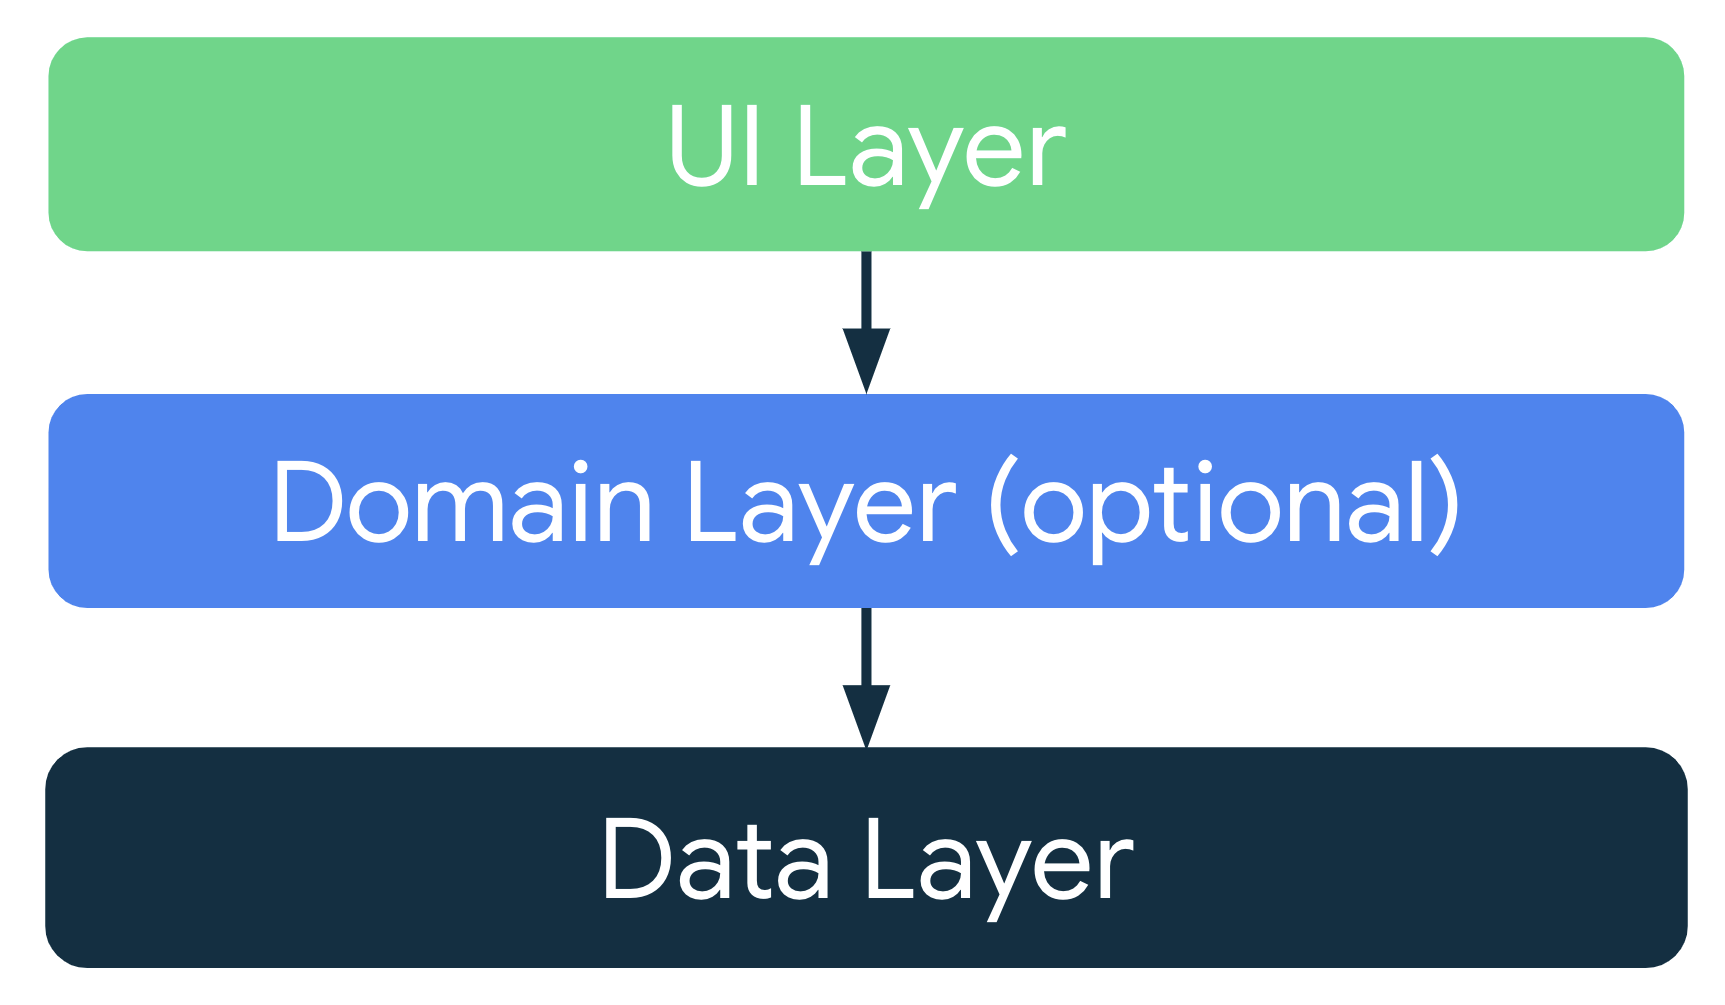
\includegraphics[width=0.5\linewidth]{android-architecture-overall}
	
	\caption{Architektura pro mobilní aplikaci pro Android \cite{android-architecture}}
	\label{fig:android-architecture-overall}
\end{figure}

\noindent Architektura je rozdělená na UI vrstvu, doménovou vrstvu a datovou vrstvu. UI (také prezentační) vrstva má na starosti zobrazení dat do uživatelského rozhraní. Uživatelské rozhraní je aktualizováno na základě událostí (např. kliknutí na tlačítko) nebo externích vstupů (odpověď ze síťového volání). UI vrstva je složena z UI elementů a držitelů stavu, jak je ilustrováno na následujícím obrázku:

\begin{figure}[H]
	\centering
	
	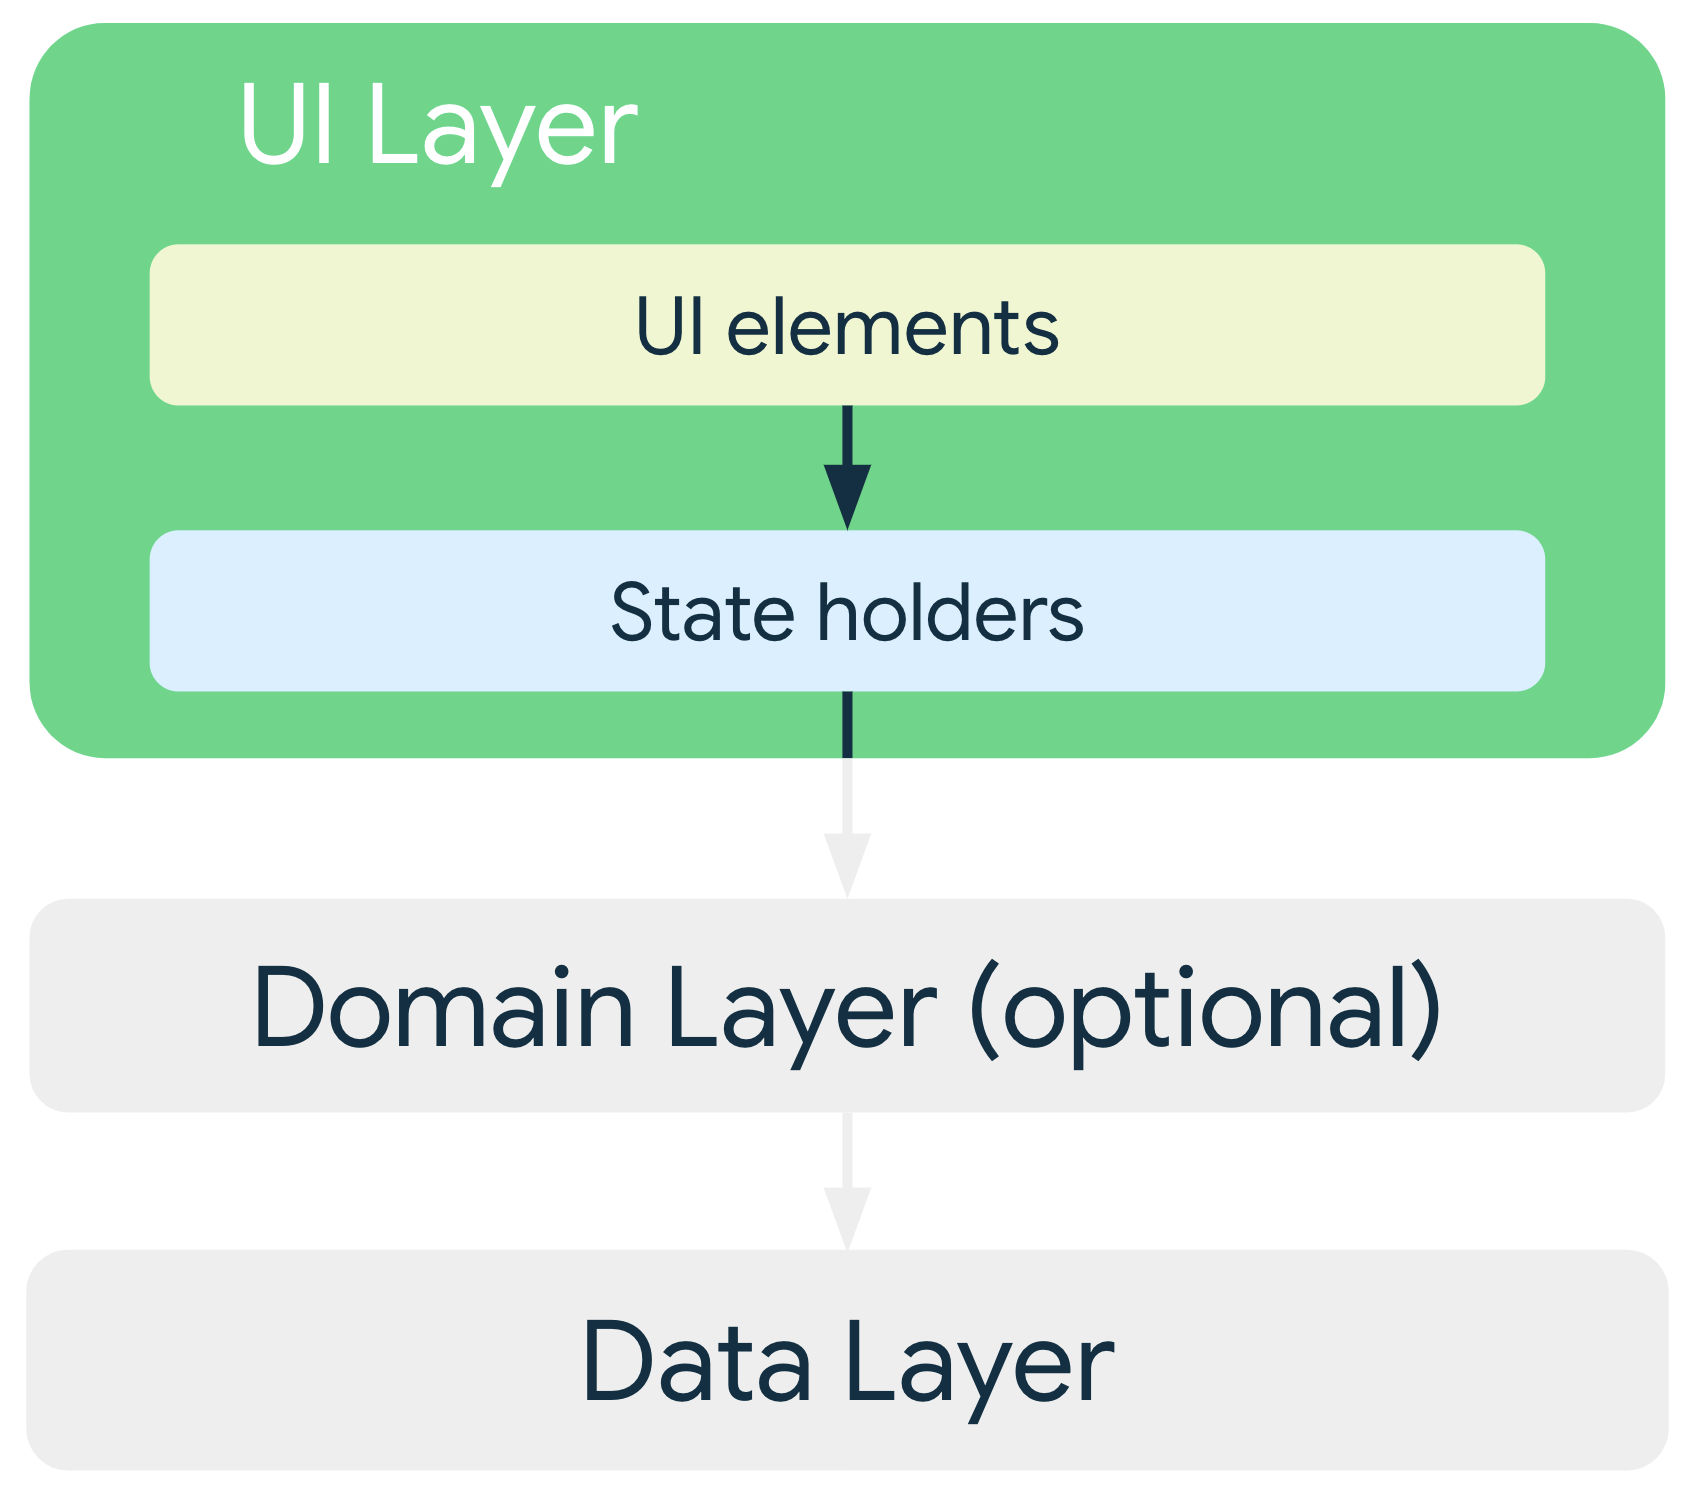
\includegraphics[width=0.5\linewidth]{android-architecture-ui}
	
	\caption{Složení UI vrstvy \cite{android-architecture}}
	\label{fig:android-architecture-ui}
\end{figure}

\noindent UI elementy reprezentují elementy, které jsou vykreslovány obrazovku. Držitelé stavu mají na starosti správu dat a aplikační logiku. Změna dat v držiteli stavu způsobi změnu UI elementů a znovu vykreslení obrazovky. Datová vrstva, jak ilustruje následující obrázek, je složena z repozitářů \linebreak  a datových zdrojů. Repozitář má na starosti vystavení dat pro zbytek aplikace, abstrahování od konkrétního způsobu získávání dat (např. jestli jsou data získávána z lokální databáze nebo vzdálěně) a centralizaci dat.  Centralizace dat slouží pro vytvoření jednotného zdroje \linebreak pravdy, tj. data jsou zbytkem aplikace vždy čerpána přímo i nepřímo z toho zdroje. Datový zdroj pak reprezentuje konkrétní zdroj dat, z kterého jsou získávána data. Může to být \linebreak např. lokální soubor, backend nebo lokální databáze. 

\begin{figure}[H]
	\centering
	
	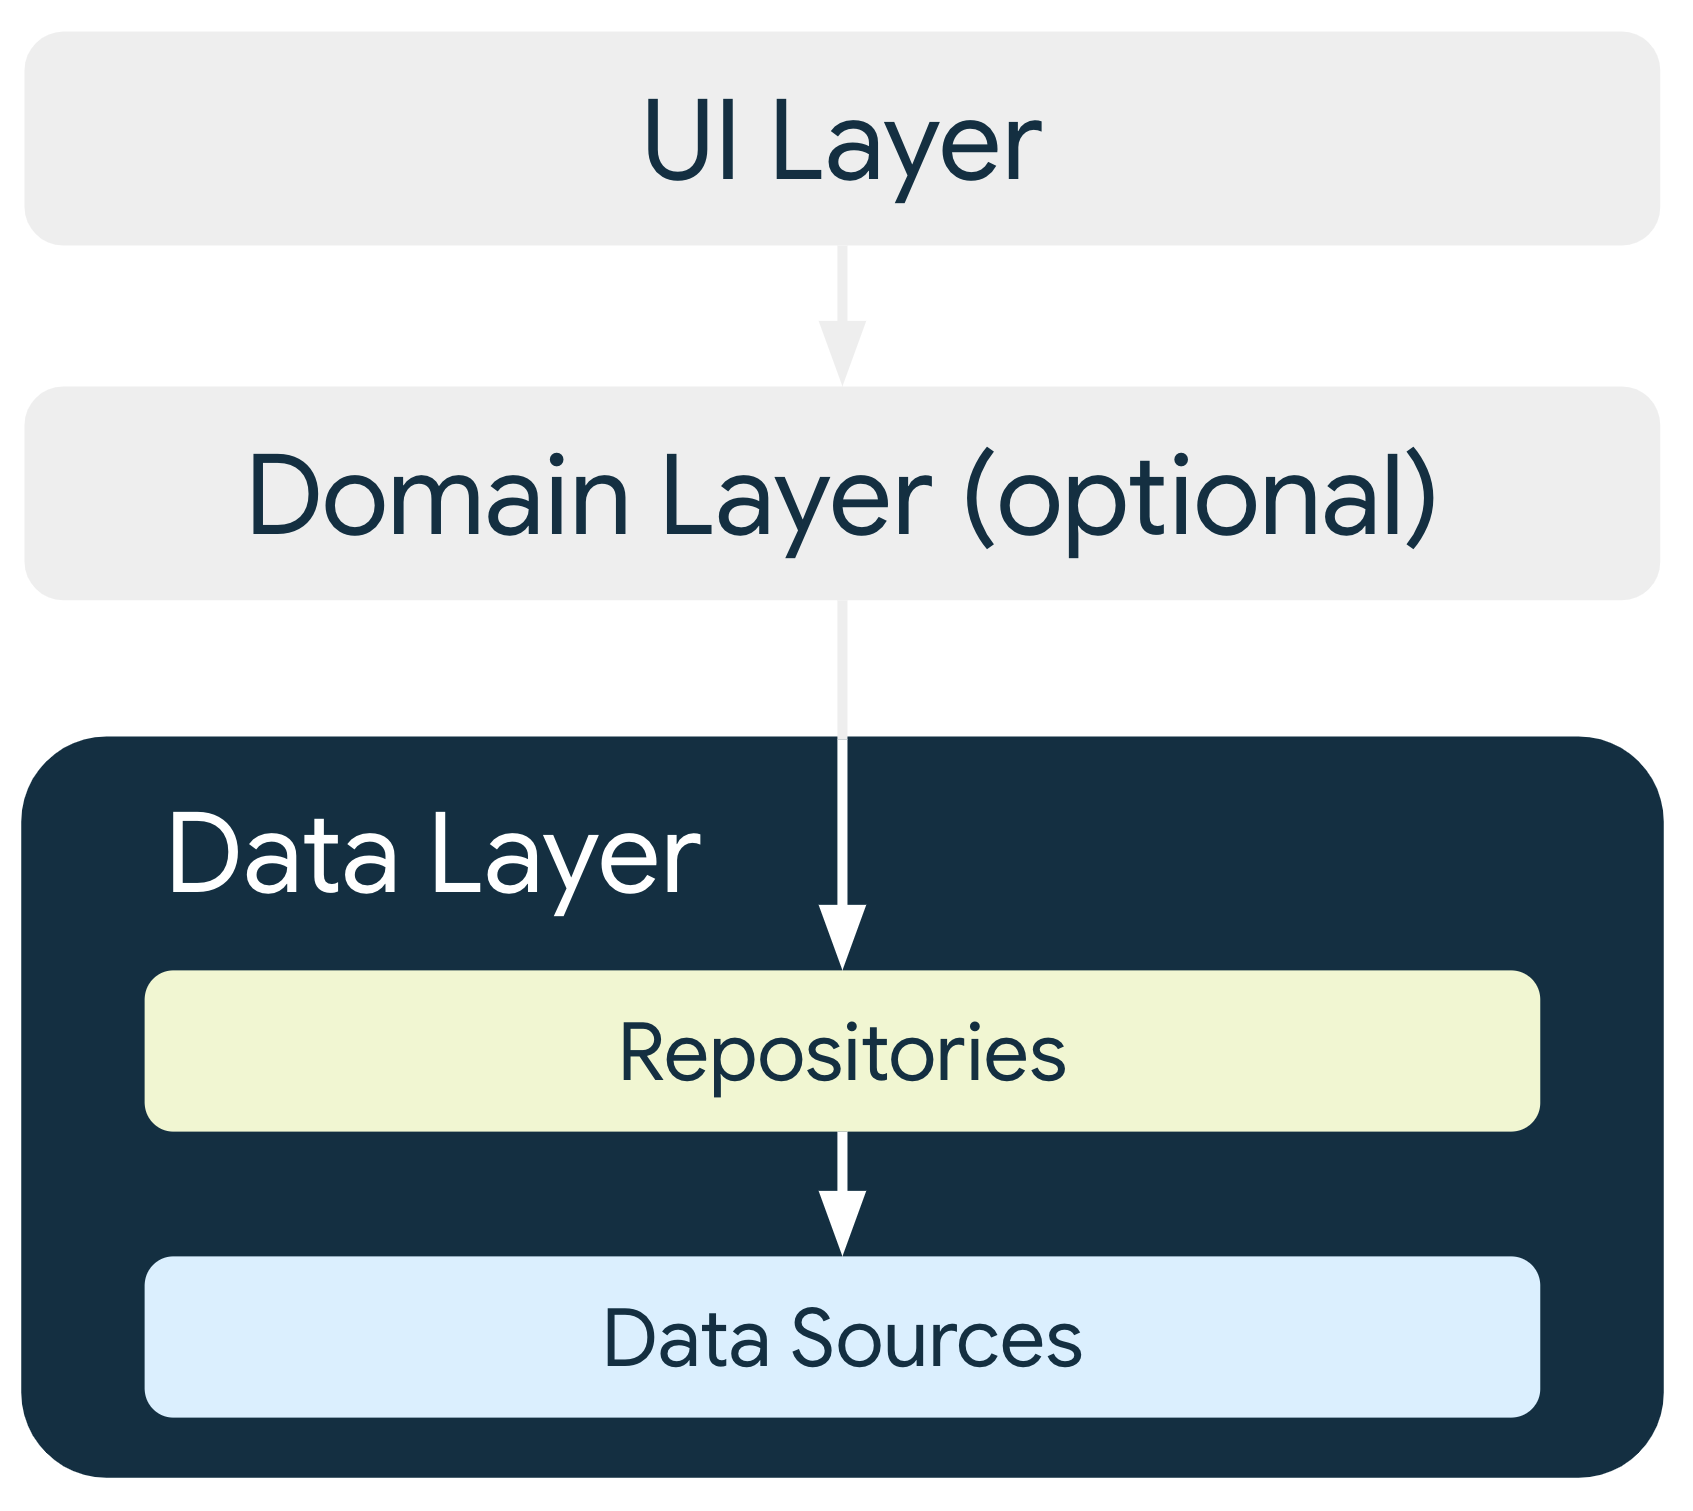
\includegraphics[width=0.5\linewidth]{android-architecture-data}
	
	\caption{Složení datové vrstvy \cite{android-architecture}}
	\label{fig:android-architecture-data}
\end{figure}

\noindent Doménová vrstva má na starosti zapouzdření složité business logiky nebo business logiky přepoužívané v několika držitelích stavu. Třídy v této vrstvě jsou obvykle pojmenovány jako \textit{use cases} nebo \textit{interactors}.

\subsection{Zhodnocení}
Architektura doporučená Googlem má následující výhody:

\begin{itemize}
	\item \textbf{Oddělení zodpovědnosti} - Rozdělení aplikace do vrstev zlepšuje udržitelnost aplikace.  Vrstvy mají mezi sebou pevně definované rozhraní. Změna implementace jedné vrstvy bude mít minimální vliv na ostatní vrstvy.

	\item \textbf{Řízení UI podle stavu dat} - Uživatelské rozhraní automaticky reaguje na změnu stavu dat. 

	\item \textbf{Jednotný zdroj pravdy} - Zajišťuje konzistenci dat.

	\item \textbf{Jednosměrný tok dat} - Data putují pouze zeshora dolu (např. z datového zdroje k repozitáři, z repozitáře k držiteli stavu). Události putují pouze zezdola nahoru (např. z UI elementů k držitěli stavu, z držitele stavu k repoiztáři). Díky tomu je fungování aplikace predikovatelné a snadno debugovatelné.

	\item \textbf{Je doporučený Googlem} - Architektura je díky tomu obecně známá. Když by na této práce začal pracovat jiný Android vývojář, vyznal by se díky této architektuře v kódu lépe.
\end{itemize}

\noindent Z těchto důvodů byla pro implementaci mobilní aplikace vybrána tato architektura. 

\section{Backend}

\subsection{5-vrstvá architektura}
5-vrstvá architektura \cite{5-tier} rozděluje aplikaci do následujících vrstev:


\begin{itemize}
	\item \textbf{Prezentační} - Má na starosti prezentaci dat uživatelovi a obsluhu událostí. Data získává \linebreak z aplikační vrstvy.
	
	\item \textbf{Aplikační} - Funguje jako prostředník mezi prezentační a businessovou vrstvou. Má na starosti aplikační logiku a řídí tok dat mezi různými vrstvami. Implementuje mimo jiné autentizaci, autorizaci a validaci dat.
	
	\item \textbf{Businessová} - Obsahuje businessovou logiku aplikace. Definuje operace, které mohou být prováděny na datech, a implementuje businessové procesy. Komunikuje s perzistentní vrstvou pro ukládání a získání dat.	
	
	\item \textbf{Perzistentní} - Tato vrstva má na starosti ukládání a získání dat z databáze. Slouží jako abstraktní rozhraní pro bussinessovou vrstvu pro přístup k datům. Data ukládá a získává komunikací s API databáze poskytované databázovou vrstvou.
	
	\item \textbf{Databázová} - Má na starosti ukládání dat. Může být implementovaná např. pomocí relační databáze. Poskytuje data perzistentní vrstvě.
	
\end{itemize}

\noindent U větších projektů lze projekt také rozdělit podle funkcionalit (např. funkcionalita pro poskytování informací o hlasování a funkcionalita pro poskytování informací o poslancích) a v rámci těchto funkcionalit použít více vrstvou architekturu.

\subsection{Architektura mikroslužeb}
Architektura mikroslužeb je architektonický styl, který rozděluje aplikaci do služeb, což jsou komponenty s následujícími vlastnostmi:

\begin{itemize}
	\item \textbf{Samostatně nasaditelné} - Každou službu lze nasadit zvlášť od ostatních služeb

	\item \textbf{Volně propojené} - Služby komunikují mezi sebou prostřednictvím API, a nejsou tedy závislé na implementaci ostatních služeb.
	
	\item \textbf{Rozdělené podle domény} - Každá služba má na starosti nějakou doménu v byznysu. \linebreak Např. jedna služba má na starosti účetnictví a jiná má na starosti objednávky.
	
	\item \textbf{Vývoj v několika týmech} - Jednotlivé služby lze vyvjíet nezávisle na ostatních \linebreak službých, pokud je zachováno API mezi nima.
	
	\item \textbf{Dobře testovatelné a udržitelné} - Každou službu lze testovat a udržovat zvlášť.
\end{itemize}

\subsection{Zhodnocení}
5-vrstvá architektura je pro účely této práce dostačující. Prezentační vrstvu bude použita pro vystavení endpointů REST API. Aplikační vrstva nebude pro jednoduchost \linebreak implementována, a místo toho budou její zodpovědnosti implementovány v rámci businessové vrstvy. Businessová vrstva bude sloužit pro abstrahování prezentační vrstvy od perzistentní vrstvy a validaci dat. Backend nebude mít téměř žádnou business logiku, bude pouze zpracovávat data z webu PSP a vystavovat je prostřednictvím REST API. Perzistentní vrstva bude použita pro abstrakci businessové vrstvy od databázové. To usnadní práce s databází. V rámci databázové vrstvy budou ukládáná data. Chybí tu však jedna další vrstva pro pravidelnou aktualizaci databázové vrstvy. Backend bude totiž pravidelně stahovat data z webu PSP a aktualizovat databázi. K této architektuře tedy bude navíc přidána \textbf{vrstva pro synchronizace databáze}.

Architektura mikroslužeb se hodí pro velké projekty, kde je předpokládáno, že budou často přicházet nové požadavky o nové funkcionality v různých částech backendu. V takovém případě je dobré backend rozdělit do nezávislých částí a ty vyjíjet, testovat, nasazovat a udržovat zvlášť v několika týmech. Nevýhodou je větší komplexita projektu. Pro účely této práce stačí toto rozdělení není potřeba, jelikož požadavky jsou předem dané a nepředpokládá se, že se budou \linebreak v budoucnu měnit. Všechny části backendu tedy budou mezi sebou komunikovat prostřednictvím programového rozhraní, nikoliv API.


